In this section, six applications are presented to illustrate the versatility of \bioptim and give a practical overview on how to use its main features.
The settings and performances (convergence time, single shooting integration error, optimized objective) of each OCP are summarized in Tab.~\ref{tab:Perfs_and_detailed_implementations_of_each_example}. 
When possible, problems were solved with both \ipopt and \acados.
In the following, bold symbols denote vectors and starred ones ($^*$) denote reference or tracked quantities.


\subsection{Muscle activation driven pointing task}\label{ex:poiting}
%
In this first example, the goal was to achieve a muscle activation driven pointing task using a 2-DoF arm model with six muscle elements. 
In addition to muscle-induced torques, pure joint torques were added to compensate for the model weaknesses.
The main term (highest weight) of the objective function (Eq.~\ref{eq:cost_pointing}) is a Mayer objective, corresponding to the pointing tasks at the final node, to superimpose two markers, the first one ($\mathbf{m_u}$) fixed in the ulna system of coordinates and the second one ($\mathbf{m^*_s}$) fixed in the scene.
The three Lagrange terms  were added for control (muscle activation $\bf{a}$ and joint torques $\boldsymbol{\tau}$) and state ($\bf{x}$) regularization:
\[
\begin{aligned}
	\mathcal{J} = 	&~\omega_1~\underbrace{\|\mathbf{m_u}(T)-\mathbf{m^*_s}\|^2}_{\mathtt{TRACK\_MARKERS}}~\\
	&\int_{t=0}^T\underbrace{\|\bf{a}\|^2}_{\mathtt{MIN\_ACTIVATION}}~
	+\underbrace{\|\boldsymbol\tau\|^2}_{\mathtt{MIN\_TORQUE}}~
	+\underbrace{\|\bf{x}\|^2}_{\mathtt{MIN\_STATE}}~ dt,
\end{aligned}
\addtag
\label{eq:cost_pointing}
\]

\noindent where $T\!=\!\SI{2}{\second}$ is the duration of the motion, and $\omega_1\!=\!1e5$.
The problem was discretized using 50~shooting nodes with a 5-steps Runge-Kutta-4 (RK4) integration in-between.
The problem was solved using \ipopt (with exact Hessian computations) and \acados (with a Gauss-Newton approximation of the Hessian) resulting in two very close solutions.
\acados was about 50 times faster than \ipopt and was better at enforcing the continuity constraints (as shown by the single shooting error in Tab.~\ref{tab:Perfs_and_detailed_implementations_of_each_example}).
\ipopt however ended up with a smaller optimized objective (20.8 \textit{vs} 23.2), leading to a more optimal solution than \acados. 
Superimposed snapshots of the optimal motion found with \acados are displayed in Fig.~\ref{fig:snapshots_activation_driven_pointing}.
It is worth mentioning that for the purpose of this illustration, no constraint was given on the shoulder range of motion to ensure physiological muscle trajectories. 


\subsection{Quaternion base twisting somersault}\label{ex:somersault}
In this example of acrobatic sports biomechanics, the goal was to maximize the twist rotation ($\phi$) of a 8-DoF model in a backward somersault.
The model was composed of a 6-DoF root segment and two 1-DoF torque actuated shoulder joints.
Two different numerical description of the root segment rotations were used (Euler angles and quaternions).
The objective function was as follows:

\begin{eqnarray}\label{eq:ocp_Trampo}
\mathcal{J} = \omega_1 \underbrace{\int_0^T \dot{\phi}~dt}_{\mathtt{MIN\_TWIST}}  +~\omega_2 \underbrace{\int_0^T \sum_{i=1}^{2}~\tau_{i}^2~dt}_{\mathtt{MIN\_ TORQUE}},
\end{eqnarray}
with $\omega_1 = -1$ (resulting in the maximization of the first term) and $\omega_2 = 1\times 10^{-6}$, T the duration of the movement and $\tau_{i}$ the torque control input of the $i^{th}$ arm DoF.
The first term of the objective function (Eq.~\ref{eq:ocp_Trampo}) corresponds to maximizing the twist velocity and the second term serves as control regularization.


The movement lasted for approximately 1 second and was discretized with 80 shooting nodes.
The solutions for both models were \comment{similar}{ce n'est pas vraiment le cas, commenter} (Fig.~\ref{fig:snapshots_quaternion_base_twisting_somersault}) highlighting the equivalence of the two rotation representations.
Euler angles have the advantage to be easily interpretable, but they suffer from the loss of a DoF at the Gimbal lock (leading to numerical instabilities).
The use of a quaternion-based representation is tackles this numerical stability issue when a joint is free to rotate on a three-dimensional range of motion.
Quaternion's integration must be handled with care~\cite{bailly2020optimal}, which was taken care of in \textit{bioptim}.


\begin{figure*}[t!]
\centering
\includegraphics[width=\textwidth]{figures/Euler_Bioptim_MaxVrille_dos.png}\\
\vspace*{0.5em}
\includegraphics[width=\textwidth]{figures/Quat_Bioptim_MaxVrille_dos.png}
\caption{Snapshots of a maximally twisting somersault driven by shoulder torque actuators and a free base expressed by Euler angles (top) or quaternions (bottom).}
\label{fig:snapshots_quaternion_base_twisting_somersault}
\end{figure*}


% \begin{table}[h!]
% \caption{\small Objective terms of quaternion base maximally twisting somersault}
% \label{tab:Quaternion_base_twisting_somersault}
% \centering
% \begin{tabular}{c c c c}
% \toprule 
% & Type & Function & Weight \\ 
% \midrule
% $\#1$ & Lagrange & MINIMIZE\_TWIST & $-1e1$ \\ 
% \midrule
% $\#2$ & Lagrange & MINIMIZE\_ TORQUE & $1e-6$ \\ 
% \bottomrule
% \end{tabular}
% \end{table}















\subsection{Pendulum on a spring}\label{ex:spring}
\emph{\begin{figure}[t!]
\centering
\includegraphics[width=0.35\columnwidth]{figures/Mass_Pendulum_Model_2.png}
\caption{Definition of the spring-mass-pendulum model.}
\label{fig:Mass_Pendulum_Model}
\end{figure}}
This spring-mass-pendulum-based example is presented to introduce \bioptim 's ability to use external forces.
The goal was to hold the position of a $\SI{1}{\kilo\gram}$ mass hanging on a linear spring attached to the ground.
A $\SI{0.2}{\meter}$-long pendulum weighting $\SI{10}{\kilo\gram}$ was attached to the mass and free to rotate in one dimension (Fig.~\ref{fig:Mass_Pendulum_Model}).
In addition to the spring force, the mass was actuated by a vertical external force (e.g., something pulling on it) while the pendulum rotation was passive.
The system therefore comprised two DoFs, the mass position ($q_m$) and the pendulum angle ($q_p$) and one control input, the vertical external force pulling on the mass ($\tau$). 
The spring force $\mathcal{F}_s$ was:
\[
\begin{aligned}
\tau_s = -k*q_m,
\end{aligned}
\addtag
\label{eq:f_ext}
\]
with $k$ the spring stiffness constant.\\
The OCP was composed of two phases each lasting for $\SI{5}{\second}$, with 50 shooting nodes.
In the first phase, no objective function was minimized and $\tau$ was constrained to be $0$, letting the mass oscillating freely. 
Then, in the second phase, a cost function (Eq.~\ref{eq:ocp_Pendulum}) was minimized, to enforce a reference position $q_m^*$ of the mass.
This objective function, exclusively composed of Lagrange terms, was formulated as follows:
\[
\mathcal{J} = \int_{T/2}^T \underbrace{ (q_m - q_m^*)^2}_{\mathtt{TRACK\_STATE}}  +~\omega_1 \underbrace{\tau^2~dt}_{\mathtt{MIN\_ TORQUE}}~dt,
\addtag
\label{eq:ocp_Pendulum}
\]

\noindent with $q_m^* = \SI{-0.5}{\meter}$ and $\omega_1 = 10^{-6}$ and T is the duration of the movement.
The first term of the objective function (Eq.~\ref{eq:ocp_Pendulum}) acts as a position controller for the mass.
The second was added for control regularization.


During the first phase, the mass is passively oscillating around its stationary position due to the spring force (Fig.~\ref{fig:Mass_Pendulum_Fext_graphs}).
At the beginning of the second phase, when an additional external force acts on the mass, it stabilizes around the targeted position.
The standard deviation between the position and the targeted position is $\SI{0.04}{\m}$.
This example highlights the possibility of using optimal control to find activation patterns compensating for external passive forces (e.g., ortheses flexibility, contact surface deformation, interaction between two models, etc.).

\begin{figure*}[t!]
\centering
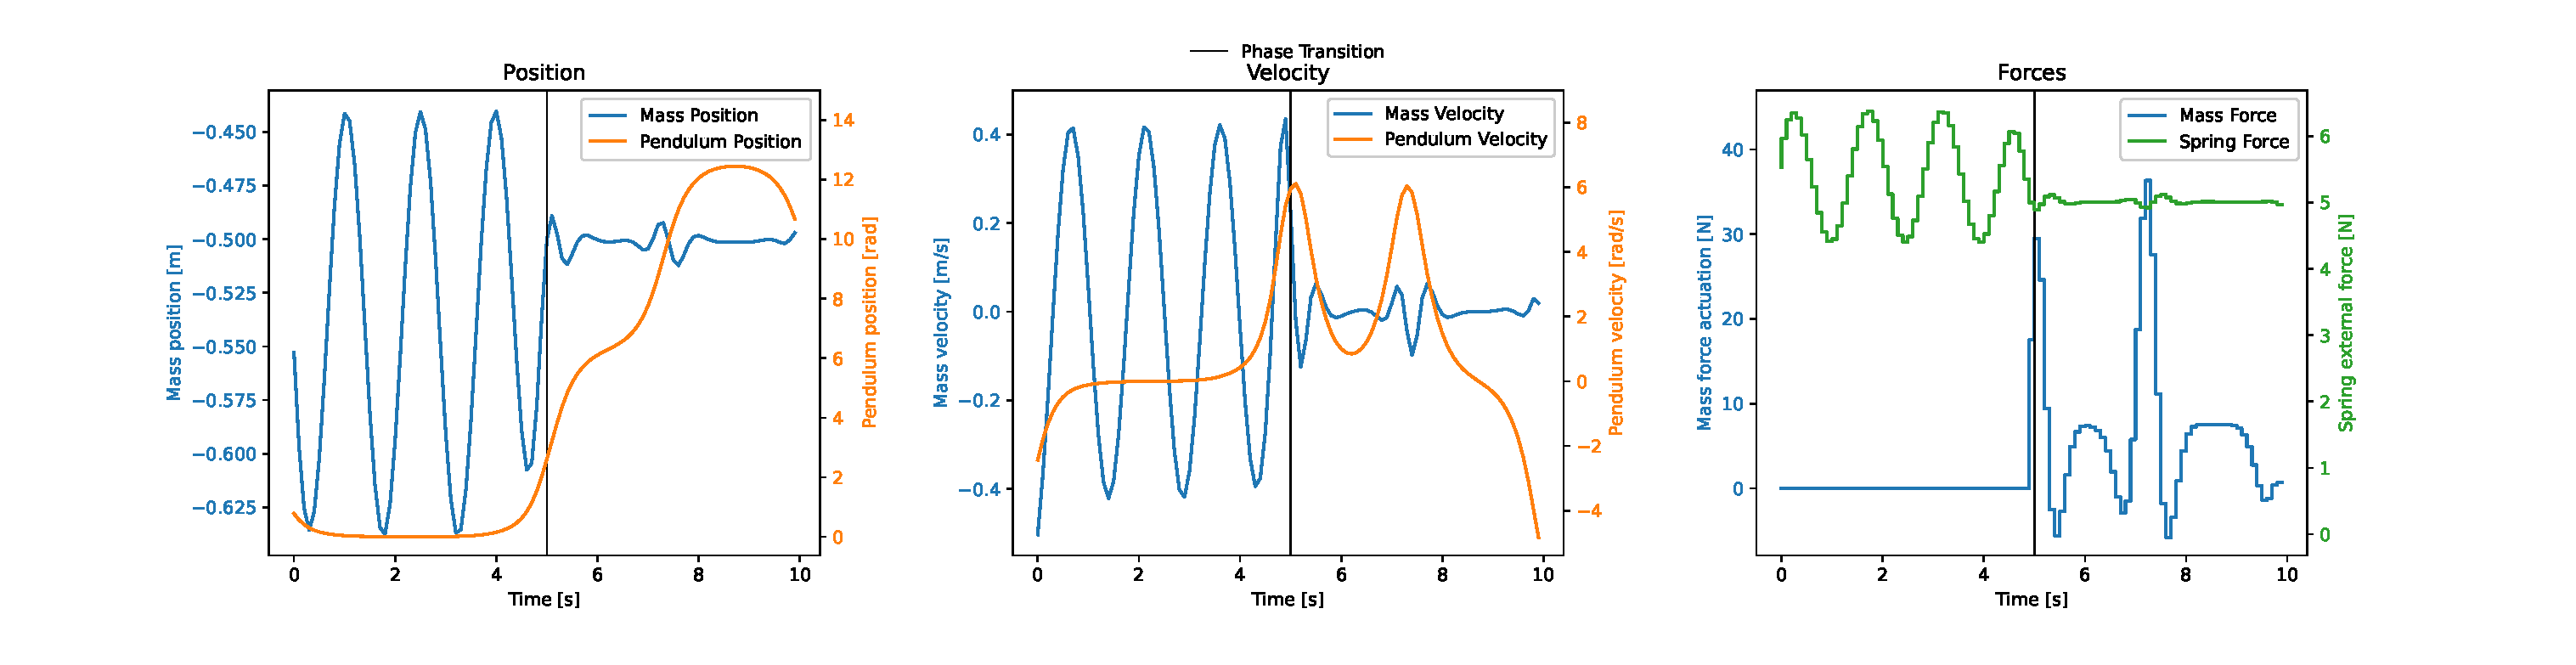
\includegraphics[width=\textwidth]{figures/Mass_Pendulum_Fext.eps}
\caption{Two-phases kinematics of the mass-pendulum-spring system. Gray dashed lines show the phase transition, blue lines are related to the mass (position velocity and external force acting on it), red lines are related to the pendulum (position and velocity) and the green line depicts the spring force.}
\label{fig:Mass_Pendulum_Fext_graphs}
\end{figure*}
















\subsection{Multiphase torque driven walking cycle}\label{ex:walking}
This walking example is presented to introduce \textit{bioptim}'s ability to deal with gait biomechanics as a multiphase problem with contact forces.
The goal was to estimate muscles activation by tracking markers trajectories, ground reaction forces and moments (Equations.~\ref{eq:ocp_markers}, ~\ref{eq:ocp_forces} and ~\ref{eq:ocp_moments}, respectively). 
The model was driven by muscle activation. 
To predict muscle activity, the objective function consisted in finding the least squared muscle activations $a_{i}$ (Equations.~\ref{eq:ocp_muscles}). 
Pure residual torques were also added to compensate potential underactuation from the model weaknesses and penalized as shown in equation ~\ref{eq:ocp_torques}.\\
The gait cycle was defined from the first heel strike to the end of the swing phase using a simplified 3D one-leg model with 12 DoFs and 17 muscles (pelvis + right lower limb). 
Based on experimental force plateform data and markers position, the stance was divided into three phases (heel, flatfoot and forefoot contacts) of fixed duration (0.05, 0.355 and 0.16s), to follow the natural rolling movement of the foot from heel strike to toe off.
The swing phase lasted 0.38 s. 
The interaction between the ground and the foot was modelled using a 4-contact points model located at the heel and the forefoot (first, fifth metatarsi and hallux).

The complete cycle was discretized in 90 intervals and the objective functions are written as follow :\\

%\[ 
%\resizebox{0.9\columnwidth}{!}{$ 
%\begin{aligned}
%\mathcal{J} = &\int_{t=0}^{T}\underbrace{\omega_1(\|m_p - m_m\|^{2})}_{\mathtt{TRACK\_MARKERS}}~ 
%+ ~ \underbrace{\omega_2(\|f_p - f_c\|^{2})}_{\mathtt{TRACK\_FORCES}}\\
%&+ ~ \underbrace{\omega_3(\|tau^f_p - tau^f_m\|^{2})}_{\mathtt{TRACK\_MOMENTS}}~
%\mathcal{J} = &\int_{t=0}^{T}\underbrace{\omega_1(\|m_p - m^*_m\|^{2})}_{\mathtt{TRACK\_MARKERS}}~ 
%+ ~ \underbrace{\omega_2(\|f_p - f^*_c\|^{2})}_{\mathtt{TRACK\_FORCES}}\\
%&+ ~ \underbrace{\omega_3(\|tau^f_p - tau^{f*}_m\|^{2})}_{\mathtt{TRACK\_MOMENTS}}~
%+ ~ \underbrace{\omega_4\|a\|^2}_{\mathtt{MIN\_ACTIVATION}}~dt, 
%\end{aligned}  
%$}  
%$}
%\addtag  
%\label{eq:ocp_walk}  
%\]

\begin{eqnarray}
\label{eq:ocp_markers}
\mathcal{J} = \sum_{i=1}^{N_i}\Bigg(\underbrace{\omega_1(\|m_p - m_m\|^{2})}_{\mathtt{TRACK\_MARKERS}}
\end{eqnarray}
\begin{eqnarray}
\label{eq:ocp_forces}
+ \underbrace{\omega_2(\|\sum_{c=1}^{N_c}F_p - F_m\|^{2})}_{\mathtt{TRACK\_FORCES}}
\end{eqnarray}
\begin{eqnarray}
\label{eq:ocp_moments}
+ \underbrace{\omega_3(\|\sum_{c=1}^{N_c}M_p - M_m\|^{2})}_{\mathtt{TRACK\_MOMENTS}}
\end{eqnarray}
\begin{eqnarray}
\label{eq:ocp_muscles}
+ \underbrace{\omega_4\int_0^T \sum_{i=1}^{N_i}~a_{i}^2~dt}_{\mathtt{MINIMIZE\_ ACTIVATION}})  
\end{eqnarray}
\begin{eqnarray}
\label{eq:ocp_torques}
+ \underbrace{\omega_5\int_0^T \sum_{i=1}^{2}~\tau_{i}^2~dt}_{\mathtt{MINIMIZE\_ TORQUE}}\bigg)
 \end{eqnarray}

where $\omega_{i}$ are the weighting factors ($\omega_1$=1e5, $\omega_2$=0.1, $\omega_3$=0.1, $\omega_4$=10, $\omega_5$=1), $T$ is the the duration, $N_i$ and $N_c$ are the number of time frames and contact points of the current phase. The indices $_p$ and $_m$ stand for predicted and measured data.\\

Non-slipping ($\mathtt{NON\_SLIPPING}$) and unilateral contact force ($\mathtt{CONTACT\_FORCE}$) constraints prevented the foot from slipping and pulling from the ground. 
In between phases, the use of the $\mathtt{IMPACT}$ state transition allowed to represent the gain or loss of contact(s) in the dynamics (e.g., swing phase to heel strike [thesis Felis - articles?]) \\

Fig.~\ref{fig:snapshots_multiphase_walking_cycle} shows the leg movements during the walking cycle. The mean tracking error on markers trajectories was 0.027 m (mean error on pelvic and foot markers was 0.0075 m and 0.0147 m, respectively). 
Concerning ground reaction forces tracking, the mean error was 4.85 N with an average $R^2$ at 0.9. 
Gluteal muscles were only activated during the stance phase and especially during the early flatfoot phase for the gluteus maximus with a maximal activation of 0.2. 
For the thigh muscles, the semimembranous, semitendinous and biceps femoris were activated during the early stance phase and terminal swing (maximal activation of 0.3, 0.4 and 0.4, respectively). 
The knee extensors, vastus lateralis, medialis and intermedius followed the same pattern and were mainly activated during the flatfoot phase. 
However, maximal activation of the rectus femoris appeared at early forefoot phase and early swing. Leg muscles were highly activated (saturation of gastocnemius lateralis and medialis) at the end of the stance and the early swing phase. 

\begin{figure*}[t!]
\centering
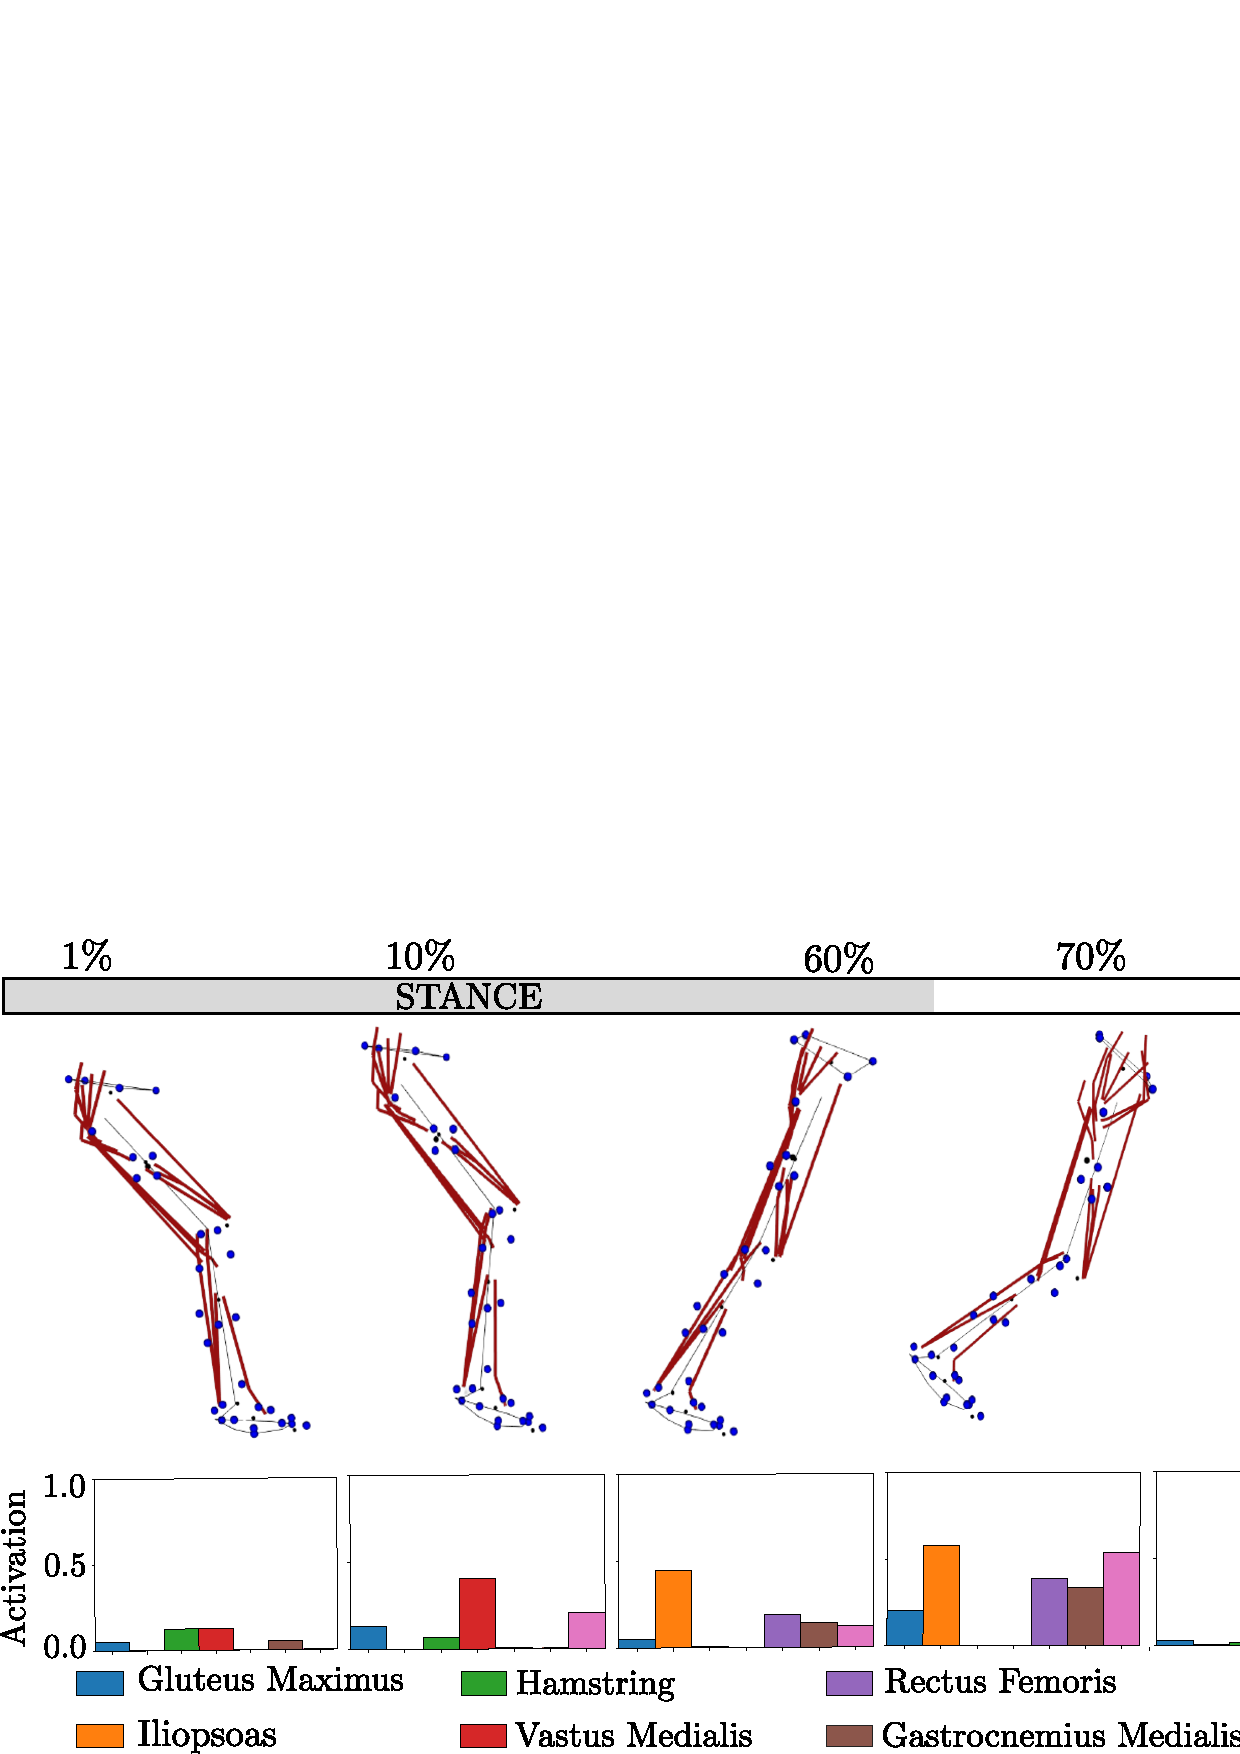
\includegraphics[width=\textwidth]{figures/multiphase_walking_cycle.png}\\
\caption{Snapshots of a walking gait cycle driven by muscles activation.}
\label{fig:snapshots_multiphase_walking_cycle}
\end{figure*}

%\begin{table}[h!]
%\caption{\small Objective terms of the Multiphase torque driven walking cycle }
%\label{tab:Multiphase_torque_driven_walking_cycle}
%\centering
%\begin{tabular}{c c c c}
%\toprule 
%& Type & Function & Weight \\ 
%\midrule
%$\#1$ & Lagrange & TRACK\_ STATE & $1e5$ \\ 
%\midrule
%$\#2$ & Lagrange & MINIMIZE\_ TORQUE\_ DERIVATIVE & $1e-2$ \\ 
%\midrule
%$\#3$ & Lagrange & TRACK\_ GRF & $1e-2$ \\ 
%\midrule
%$\#4$ & Lagrange & TRACK\_ MOMENTS & $1e-1$ \\
%\bottomrule
%\end{tabular}
%\end{table}


\subsection{Moving Horizon Estimation of Shoulder Elevation}\label{ex:mhe}
The goal was to estimate real-time joint kinematic and muscle activation using a moving horizon estimation (MHE). The example is given for a shoulder elevation motion using a 4-DoFs arm actuated by 19 Hill-type muscles. To use MHE, the OCP was split into a succession of smaller one. Each objective function was written as:

\[
\resizebox{0.9\columnwidth}{!}{$
\begin{aligned} \noindent \mathcal{J} = \sum_{n}^{n + n_{mhe}}\underbrace{\omega_1´(\|q_{ref} - q_{est}\|^{2})}_{TRACK\_STATE} ~ + ~ \underbrace{\omega_2\int_t^{t+t_{mhe}} \sum_{i=1}^{8}~Q_{i}^2~dt}_{MINIMIZE\_ STATE} ~ + ~ \underbrace{\omega_3\int_t^{t+t_{mhe}} \sum_{i=1}^{19}~U_{i}^2~dt}_{MINIMIZE\_ ACTIVATION} 
\end{aligned}
$} \addtag \label{eq:ocp_exMHE} 
\]

\noindent where $\omega_1$ =1e4 , $\omega_2$ = 10, $\omega_3$ = 100, $n_{mhe}$ is the number of OCP shooting node and $t_{mhe}$ is OCP duration. $q_{ref}$, $q_{est}$, $Q_i$ and $U_i$ are respectively reference and estimate joints angles, states and muscles activations. \\  
The first term of the objective function (Eq.~\ref{eq:ocp_exMHE}) corresponds to tracking experimental joint angles. Second and third were added for states and muscle controls regularization. Thanks to the high similarity between successive problems, a warm-start strategy using previous solutions was implemented.  
 
 
The shoulder elevation movement was generated with co-activation on two antagonists' muscles groups (triceps, biceps). It lasted for 8s and was discretized using 800 shooting nodes. A windows size of 7 nodes which allows the estimator to run around 50Hz, four times faster than standard biofeedback (13Hz), was chosen. Whereas reference data were generated at 100Hz, only one in two frames was sent to the estimator to correspond with experimental conditions.
 
The estimator was able to forecast the movement kinematic (Fig.~\ref{fig:angulare_angle_MHE}) with a consistent dynamic (Fig.~\ref{fig:muscles_excitations_MHE}). Due to cocontraction, the estimated muscles activations are lower than reference motion activations but with similar pattern. 
\begin{figure*}[t!] 
\centering 
\includegraphics[width=\textwidth]{figures/joint_angles_MHE.pdf}\\ 
\caption{Time series of estimated joint angles (blue) and noisy reference joint angles (orange).} 
\label{fig:joint_angles_MHE} 
\end{figure*} 

\begin{figure*}[t!] 
\centering 
\includegraphics[width=\textwidth]{figures/Muscle_Forces_MHE.pdf}\\ 
\caption{Time series of estimated muscle forces (blue) and ground truth muscle forces (orange). 
Only the muscles with significative action (peaks force $>$ 15~N) are represented.
Muscle abbreviations stand for (from left to right and top to bottom): Triceps Long head, Lateral and Medial, Brachial, Brachioradialis, Deltoid Anterior and Middle, Infraspinatus, Subscapularis, Biceps Brachial Long and Short head.} 
\label{fig:muscle_forces_MHE} 
\end{figure*} 


\subsection{Multiphase vertical jumper}\label{ex:jump}
This example is presented to introduce \textit{bioptim}'s ability to \hl{XXX}.
The goal was to find a minimal-time push-off phase for a \hl{XXX-DoF torque-driven} model while maximizing its jump height ($h$).
The push-off (impulsion before take-off) was divided into two phases with the following properties: \textit{1)} two contact points (heel and toe), duration $\in [0.2, 1.0]s$ and \textit{2)} one contact (toe), duration $\in [0.05, 1.0]s$.
The joint actuators bounds were modeled using a custom nonlinear constraint to account for torque/angle/angular-velocity relationships using the \verb?gauss3p? function of \textit{biorbd} \comment{based on predetermined factors}{je ne comprends pas} (\ref{fig:graph_force_vitesse_longueur}).
For each phase, the objective function was formulated as follow:

\[
\mathcal{J} = XXX.
\addtag
\label{eq:cost_jumper}
\]

The first term of Eq.~\ref{eq:cost_jumper} corresponds to maximizing the jump height.
The second term of the objective function serves for finding a minimal-time solution.

Using \textit{ipopt}, the problem was first approximately solved using the BFGS hessian approximation for 200 iterations maximum.
Then, \comment{if this maximum number of iterations was reached}{ne parler que de la solution présentée. Est-ce que le max_iter a effectivement été atteint ?}, the solution was re-optimized, using a warm-start, with exact-hessian computations for up to 1000 iterations .

The optimized ump height was 1,35m in \hl{XXX}s.
\comment{The used strategy is XXX with a proximo-distal shift of the joints (hip, knee then ankle) highlighted by the activation of the hip, then the knee and finally the ankle.}{à terminer}

\begin{figure}[h!]
\includegraphics[width=\columnwidth]{figures/graph_force_vitesse_longueur.png}\\
\caption{Surface representing the nonlinear constraint which account for torque/angle/angular-velocity relationships in the model of the jumper.}
\label{fig:graph_force_vitesse_longueur}
\end{figure}

%
\begin{table*}[h!]
\caption{\small Overview of computational results for the different OCPs cases and links to detailed implementations. The single shooting state trajectory is obtained by forwardly integrating the initial state with the optimized control inputs during 1~second. The single shooting error is computed as the mean RMSE between the optimized state vector and the single shooting one at 1~second.}
\label{tab:Perfs_and_detailed_implementations_of_each_example}
\centering
\begin{tabular}{c l rl rl rl}
\cmidrule[\heavyrulewidth](lr){2-8}
& & \multicolumn{2}{l}{\ref{ex:poiting} Activation-driven pointing} & \multicolumn{2}{l}{Ex\# 2} & \multicolumn{2}{l}{Ex\# 3} \\
\cmidrule[\heavyrulewidth](lr){3-4}
\cmidrule[\heavyrulewidth](lr){5-6}
\cmidrule[\heavyrulewidth](lr){7-8}

\mymultirow{4}{Setup} & \# states $\xt$            & \multicolumn{2}{c}{4}  & --    & --     & --    & --\\
                      & \# control $\ut$           & \multicolumn{2}{c}{6}  & --    & --     & --    & --\\
                      & \# shooting nodes          & \multicolumn{2}{c}{50} & --    & --     & --    & --\\
                      & OCP duration (s)           & \multicolumn{2}{c}{2}  & --    & --     & --    & --\\
                      &                            & \ipopt  & \acados        & \ipopt  & \acados  & \ipopt  & \acados \\
\mymultirow{3}{Solve} & \# NLP iterations          & 47     & 19            & --    & --     & --    & --\\
                      & Optimized cost             & 20.8 & 23.2        & --    & --     & --    & --\\
                      & Time to convergence (s)    & 22.3    & 0.45          & --    & --     & --    & --\\
                      & Single shooting error    & $<10^{-7}$    & $<10^{-13}$          & --    & --     & --    & --\\
%Example & Link & IPOPT & ACADOS \\ 

%\midrule
%Muscle activation driven pointing task & \href{https://github.com/pyomeca/BiorbdOptim/blob/master/examples/muscle_driven_ocp/static_arm.py}{$\star$} & $10.10$ & $0.2018$  \\ 
%\midrule
%$\bullet$ & $\bullet$ & $\bullet$ & $\bullet$ \\ 
\cmidrule[\heavyrulewidth](lr){2-8}
\end{tabular}
\end{table*}
%







